\chapter{Documentation}
The remaining chapter is dedicated to the documentation of Aphantasia.

\section{User Documentation}
\label{chap:user_documentation}
All of the pages are accessible from the homepage and/or the collapsable navbar in the top right.

\subsection{Registering and Logging in}
While not logged in, only the graph view, about page, and welcome page are accessible.

To register, click on the register button on the home screen.
The registration requires selecting a unique username, email, and password.
The password has security requirements which are displayed immediately
after opening the form and in case of not meeting the criteria on submit.

To log in click on the login button on the homescreen. The login requires a username or email and password.

At this point, the email is not used anywhere and is only included in preparation for email verification functionality.

\subsection{Opening a Thought}
There are multiple ways to open a thought:
\begin{itemize}
  \item \textbf{New thoughts log on homepage} - On the homepage, there is a feed of the last three thoughts created on the website.
 Clicking on one of them will open the thought in graph view.
  
 Clicking on the "All Thoughts" button under the feed leads to the list of all thoughts.
  \item \textbf{Notifications} - The Notifications button and the bell icon in the navbar lead to the list of replies.
 Replies are thoughts of other users linked to any of the logged-in user's thoughts.
 Clicking on a reply opens the respective thought.
  \item \textbf{Graph view} - The main way to access thoughts is through the graph view. We will take a closer look at it in the next section.
  \item \textbf{Direct link} - Every thought has a unique ID which can be shared and accessed directly using the URL in format '/graph/\{thoughtId\}'.

 Example of the full URI leading to the thought with ID 1: https://aphantasia.io/graph/1
\end{itemize}

\subsection{Graph View}
To access the graph view, click the "Graph" button on the main page
or click on the graph icon in the navbar (three connected nodes).

In the graph view, the following controls are available:
\begin{itemize}
  \item \textbf{Mouse wheel or bottom right buttons} - Zooms in and out

 Once zoomed past a threshold, titles of the thoughts appear. (Figure \ref{obr:afantazie_floating_titles})
  \item \textbf{Draging the background} - Pans the viewport
  \item \textbf{Dragging a node} - Moves the grabbed thought around
  
 This is useful for customizing the layout, "untying" thoughts that are too close to each other or to speed up the process of the layout algorithm. 
  \item \textbf{Clicking a node} - Highlights a thought and switches to highlighted mode.
\end{itemize}

\subsubsection*{Highlighted Mode}

In default mode, the whole display is used to view the graph, and the user can interact with it as described above.
When a thought is accessed, the graph view switches to highlighted mode. (Figure \ref{obr:afantazie_mobile_graph_view})

In highlighted mode half of the screen gets dedicated to the highlighted thought preview and the other half to the graph view.

The graph view in highlighted mode shares almost all behavior with the default mode, with a few exceptions:
\begin{itemize}
  \item \textbf{Visual node highlight} - The currently opened thought is also visually highlighted by a white circle around it.
  \item \textbf{Visual edges highlight} - All edges connected to the opened thought are exaggerated in thickness and color while all other edges are dimmed.
  \item \textbf{Neighborhood thoughts} - On highlighting a thought, the application loads its neighborhood.
\end{itemize}
Every time a thought is selected, the viewport also smoothly centers on it.

The thought preview shows the title, author, time of creation, content with clickable links, and replies section.
Both the links in content and titles in the replies section are color-coded based on the author's selected color, and one-click will highlight the respective thought.
At the bottom of the preview there are Reply button and a close button (up icon on mobile and X on desktop).

\subsubsection*{Neighborhood Thoughts and Graph Exploration}

When a thought is highlighted, the application loads its neighborhood.
The neighborhood is defined as thoughts accessible through \gls{BFS} up to a given depth.
The currently used depth of the search is fixed at 3.

Some of the thoughts rendered on screen can be filled with black color. \ref{obr:afantazie_mobile_graph_view}
This indicates that some neighbors of the node are not visible on screen, and thus, the node is explorable.
  
\subsection{Creating a New Thought}

There are two ways to access the thought creation page:
\begin{itemize}
  \item \textbf{From the graph view} - Click on the "New thought" button at the bottom of the graph view.
  \item \textbf{From the thought preview} - Click on the "Reply" button at the bottom of the thought preview.
\end{itemize}

Both of these ways lead to the thought creation page (Figure \ref{obr:afantazie_thought_creation_page}).
The difference between them is that when accessed through the Reply button, the respective thought link
is automatically added to the content input.

The thought creation page consists of two text fields: Title and Content.

Both the title and content are required. Title has a minimum length of 1 character. The content's minimum length is 5 characters.
Both of these requirements are enforced by validation rules, and the user is notified by notification messages if the submit fails.

\subsubsection*{Referencing Other Thoughts}
When a link (or a reference) is added to a thought, it will be connected and attract the corresponding node in graph view.
Links can be added to the content field as a link with the format "[id](text)",
where id is the id of the thought and text is the text that will be displayed.
The text does not have to necessarily be the original title of the linked thought.

Adding links can be done in three ways:
\begin{itemize}
  \item \textbf{Manually} - By typing the link in the content field
  \item \textbf{By 'Add reference' button} - This button opens an overlay with a list of thought titles and a search bar.
 Click on a thought title to add it to the content at the cursor position.
  \item \textbf{Reply} - As mentioned, the Reply button in the graph view adds the link to the respective thought automatically.
\end{itemize}

Each thought can have up to five references.

\begin{figure}[h]\centering
  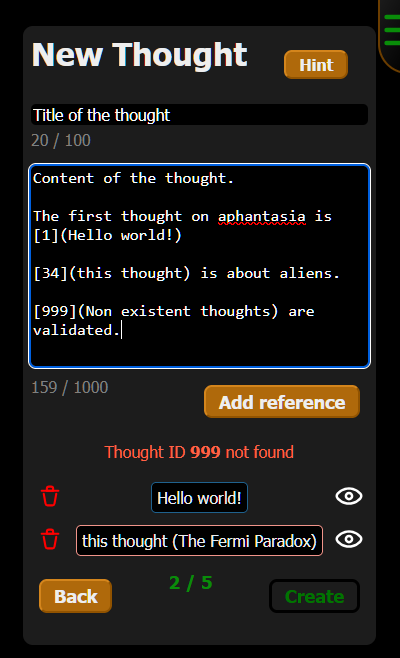
\includegraphics[width=100mm, keepaspectratio]{img/afantazie_thought_creation_page.png}
  \caption{Aphantasia - Thought creation page}
  \label{obr:afantazie_thought_creation_page}
\end{figure}

\subsection{Settings}
The settings page (Figure \ref{obr:afantazie_user_settings}) is accessible from the navbar by clicking on the gear icon or by clicking the "User settings" button on the homepage.
Currently, there are two settings that can be changed:
\begin{itemize}
  \item \textbf{On-screen thought limit} - This setting changes the maximum number of thoughts that are displayed on screen at once.
 The default value is 100. but can be changed to virtually any positive value.
  \item \textbf{Color} - This setting changes the color of users' thoughts in the graph view.
 There are predefined colors accessible by clicking the username but users are free to choose any color they like using a hexcode.
\end{itemize}

\begin{figure}[h]\centering
  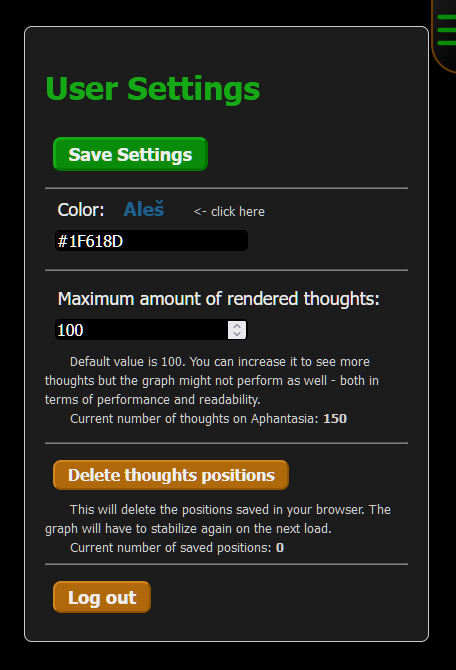
\includegraphics[width=100mm, keepaspectratio]{img/afantazie_user_settings.png}
  \caption{Aphantasia - User settings}
  \label{obr:afantazie_user_settings}
\end{figure}

Apart from these settings, there is also a \textbf{Log out} button
and \textbf{Delete thought positions} button, which erases positions of thoughts saved in the browser - forcing the graph to restabilize on the next load.

\section{Installation Guide}
Here we will look at how to set up and run both locally and how to deploy a public instance. 

\subsection{Running Aphantasia Locally}
To run Aphantasia locally, follow these steps:

\subsubsection{Database}
The database is necessary for the application to run.
It is set up using Entity Framework Core and PostgreSQL but one can choose any other database engine supported by EF Core.
To use a different database engine, install the necessary packages
and replace the \textbf{UseNpsql} methods in these two files appropriately:
\begin{itemize}
  \item \textbf{Afantazie.Data.Model/DatabaseContextProvider.cs}
  \item \textbf{Afantazie.Data.Model/DesignTimeDataContextFactory.cs}
\end{itemize}

With the database running the next step is to scaffold the database (ie. create the schema compatible with Aphantasia).
To do so, follow these steps:
\begin{enumerate}
  \item Add a file named \textbf{migrationsettings.json} in the root of project \textbf{Afantazie.Data.Model}.
  \item Add the following content to the file:
  \begin{lstlisting}
{
  "ConnectionStrings": {
    "DefaultConnection": "DATABASE CONNECTION STRING"
  }
}
  \end{lstlisting}
  \item Run the following command in the Data.Model project root:
  \begin{lstlisting}
    dotnet ef database update
  \end{lstlisting}
\end{enumerate}

The command should print the connection string provided in the migrationsettings.json and ask for confirmation.
If everything is correct, confirm the prompt by inputting "y", and the database should be created.

\subsubsection{Frontend}
Before running the frontend make sure to have Node.js with npm installed on the machine.
Open the root of the AfantazieWeb directory in a command line and run:
\begin{lstlisting}
 npm install
 npm run dev
\end{lstlisting}

The application will then be accessible at the address seen in the console output.
The language of the application can be changed by replacing \textbf{VITE\_LANGUAGE} to either 'en' or 'cz' inside the .env.development file.

\subsubsection{Backend}
Before running the backend, make sure to have .NET 8 SDK installed on the machine.

To run the Aphantasia backend, we recommend using Visual Studio and following these steps:
\begin{enumerate}
  \item Open the AfantazieServer.sln solution file in Visual Studio.
  \item Right-click the AfantazieServer project and click on Manage User Secrets.
  \item Copy the JSON with the connection string we provided in the database setup section and paste it into the secrets.json file.
  \item Set the AfantazieServer project as a startup project and run it.
\end{enumerate}

The project can be configured in the appsettings.Development.json file,
but it is not necessary for the application to run.

\subsubsection{Testing Data}
\label{sec:testing_data}
Apart from adding testing data manually throught the appliaction or directly inserting into the database one can also use the Afantazie.Tools project.
It is a .NET 8 console application inside the AfantazieServer solution
we created to help with various tasks regarding Afantazie development.
Among other things, it can generate random thoughts and users and add them to the database.

Before running the tool to generate thoughts, follow these steps:
\begin{enumerate}
  \item Host and scaffold a database as described above.
  \item Manually remove foreign key constraints from the ThoughtReferences table.
  \footnote{This is necessary as the tool doesn't generate the data optimally and violates these constraints.
 They can be added back after the import but it is not necessary for the application to run.}
  \item Create an appsettings.json in the root of the project.
 Its content should be the same as the migrationsettings.json shown above.
\end{enumerate}

Then, set the project as the startup project and run it.
Again the tool wil print the connection string and ask for confirmation after which it will present several options to pick from.
There are a few random data generators, but we recommend using option 3 - 'Generate random rainbow thoughts'.

This option will generate random clusters of thoughts where each generated thought has a set probability
of being linked to a thought in a different cluster.
User will then be asked for various parameters - fill them in and let the tool run.
Once it finishes, the database will be filled with random clustered thoughts
and users with unique colors across the color spectrum.

\subsection{Deploying Aphantasia}
To host Aphantasia publicly, we recommend using a Linux server (We used Debian 12.8).

Set up the database using the same steps as in the local setup.
The database can be hosted on the same server or on an external service (server or cloud).

\subsubsection{Frontend}
To prepare the frontend for deployment, first modify the .env.production file in the root of the AfantazieWeb directory.
Language and the backend URL need to be configured. Here is an example of our configuration:
\begin{lstlisting}
 VITE_LANGUAGE=cz
 VITE_URL=https://afantazie.cz
\end{lstlisting}

Then run the following commands in the root of the AfantazieWeb directory:
\begin{lstlisting}
 npm install
 npm run build
\end{lstlisting}

This will create a dist directory with the compiled frontend code.
Copy this code to a public directory on the server.

\subsubsection{Backend}
To deploy the backend, first, modify the app settings.Production.json file at the root of the AfantazieServer project.
Here is an example of our configuration:
\begin{lstlisting}
{
  "ApplicationLanguage": "cz",
  "JwtSecurityKey": "SECRET_KEY_HERE",

  "ConnectionStrings": {
    "DefaultConnection": "DATABASE CONNECTION STRING"
  }
}
\end{lstlisting}

In the JwtSecurityKey field, insert a secure string that will be used to sign JWT tokens.
In the ConnectionStrings field, insert the connection string to the database.
One can also change the language of the application by changing the ApplicationLanguage field.

We recommend using Visual Studio IDE to build the backend.
Create a new publish profile and set the target runtime to "Portable".
Then, publish the project in a directory and copy the files to the server.
Make sure to have the .NET 8 runtime installed on the server.

Finally, run the AfantazieServer.dll file with the following command:
\begin{lstlisting}
 dotnet AfantazieServer.dll
\end{lstlisting}

This way, the server will only run as long as the terminal is open.
To run the process in the background, we highly recommend using a program called \textbf{tmux} (another alternative is program \textbf{screen}).
Utilizing tmux makes it possible to run the server in the background.

\subsubsection{Nginx Configuration}
\label{sec:nginx_config}
As stated in Section \ref{sec:hosting} we use Nginx as a reverse proxy to reroute requests to the backend and to force the meta.json file to be always returned.
Here is how we set up the Nginx configuration file:
\begin{lstlisting}
server {
  server_name www.afantazie.cz afantazie.cz;
  root /www/hosting/afantazie.cz/www;

  index index.php index.html;

  include /etc/Nginx/sites-available/domains_conf/afantazie.cz.conf;
  if ($scheme != https) { return 308 https://$host$request_uri$is_args$args; }

  location /api {
    proxy_pass         http://127.0.0.1:5000;
    proxy_http_version 1.1;
    proxy_set_header   Upgrade $http_upgrade;
    proxy_set_header   Connection keep-alive;
    proxy_set_header   Host $host;
    proxy_cache_bypass $http_upgrade;
    proxy_set_header   X-Forwarded-For $proxy_add_x_forwarded_for;
    proxy_set_header   X-Forwarded-Proto $scheme;
  }

  location /hub {
    proxy_pass         http://127.0.0.1:5000;
    proxy_http_version 1.1;
    proxy_set_header   Upgrade $http_upgrade;
    proxy_set_header   Connection "Upgrade";
    proxy_set_header   Host $host;
    proxy_cache_bypass $http_upgrade;
    proxy_set_header   X-Forwarded-For $proxy_add_x_forwarded_for;
    proxy_set_header   X-Forwarded-Proto $scheme;
  }

  location /meta.json {
    add_header Cache-Control "no-cache, no-store, must-revalidate";
    expires -1;
  }
}
\end{lstlisting}

\section{Administrator Documentation}
This section is dedicated to the documentation of the Aphantasia administration.

\subsection{Backend}
To understand the architecture of the backend, see the detailed architecture description in Chapter \ref{sec:implementation_backend}.
There is not much to be done on the backend side apart from the initial setup and deployment.

The application has an active console logging, and one can see the activity on the site, including the number of currently active users,
thoughts currently being explored, as well as the creation of new thoughts.

\subsection{Frontend}
To understand the architecture of the frontend, see the detailed architecture description in Chapter \ref{sec:frontend_architecture}.


\subsubsection{Graph Layout Algorithm Parameters}
While running the Aphantasia's frontend publically it is important to keep in mind that the graph parametrization might become insufficient as the graph grows.
This is the main administration task on the frontend side - adjusting the graph layout algorithm parameters.

\label{sec:graph_layout_parameters}
\begin{itemize}
  \item \textbf{Forces}: Pull force, push force, and gravity force, including maximum allowed values and distance thresholds
  \item \textbf{Gravity On}: Boolean value that turns the gravity force on or off 
  \item \textbf{Link Distance}: Controls the spacing between connected thoughts
  \item \textbf{Momentum Dampening Divisor}: Forces acting on thoughts are divided by this number, resulting in a smoother with less jitter, but the graph will be slower to stabilize.
  \item \textbf{Stage Size}: The size of the simulation container
  \item \textbf{Radius Controls}: Base radius, size multiplier (how much larger more-referenced thoughts are), and maximum radius
  \item \textbf{Simulation Falloff Time}: Gradually slows down the \gls{GLA} after each user interaction (dragging or selecting thoughts and time sliding)
  \item \textbf{Frames with Overlap}: Allows newly appeared thoughts to overlap for a given amount of frames
  \item \textbf{Layout Caching Frequency}: Specifies how often the layout is saved to \gls{local_storage}
  \item \textbf{Node Mass}: Allows differently sized thoughts to have proportional influence on each other, with maximum and minimum values also parametrized
  \item \textbf{Backlinks Count Force Divisor}: Reduces forces acting on highly connected nodes
  \item \textbf{Edges Appearance}: Adjusts thickness and color of highlighted and unhighlighted edges (edges leading in or out of the currently highlighted node)
  \item \textbf{Animated Edges}: Turns on animated edges feature (seen in Figure \ref{obr:afantazie_animated_edges})
  \item \textbf{Frames With Less Influence}: New thoughts start with no influence over the simulation and gradually gain it over time
\end{itemize}